\section{Results}
This chapter will focus on providing visual representations of the findings from the experiment. These findings will be described in detail to further be used to evaluate the hypothesis in the discussion section of the report. 


\subsection{Relationship between training iterations and loss}
\begin{figure}[h]
   \centering
   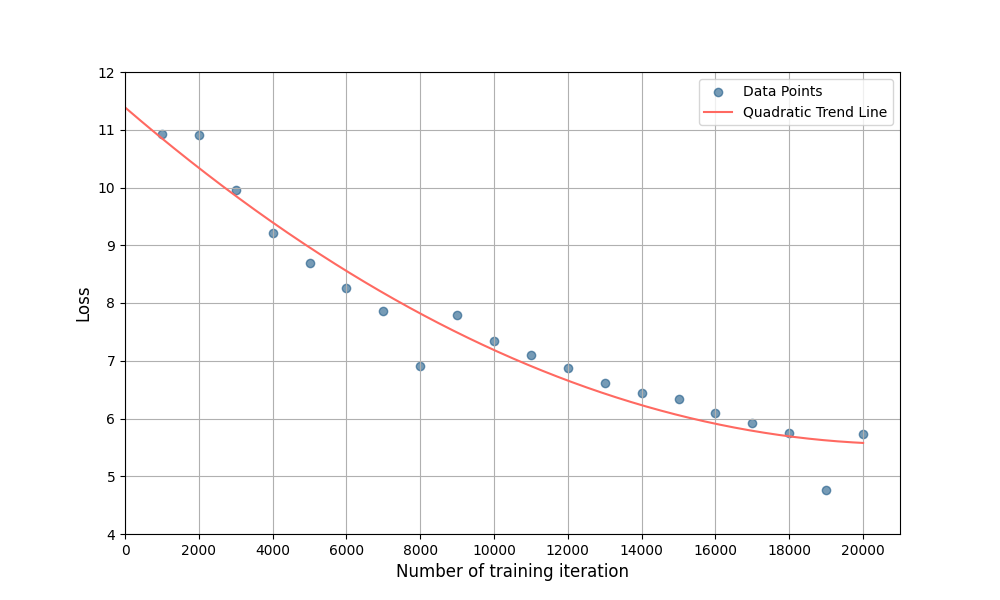
\includegraphics[width=0.9\textwidth]{../Data/loss_by_iteration_plot.png}
   \caption{Quadratic Trend Analysis of Loss Reduction Over 20,000 Training Iterations}
   \label{fig:loss-vs-training-iterations}
\end{figure}
The data illustrated in Fig.\ref{fig:loss-vs-training-iterations} displays the relationship between the the loss of the object detection model over the 20,000 training iterations of the machine learning algorithms. It can be seen that during the initial stages of the experiment, a sharp decline in the loss can be viewed. This demonstrates the initial learning phase of the program. However, with an increased number of training iterations, the rate of the loss decreasing steadily slows down as it approaches its optimal state. \\

The quadratic trendline graphed in Fig.\ref{fig:loss-vs-training-iterations}  displays the model approaching a state of convergence, as the training iteration count increases and loss decreases. Furthermore, the trendline expresses the non-linear relationship between training iterations and the loss of the model. \\
\newpage

\subsection{Relationship between training iterations and accuracy}
The accuracy per class analysis illustrates the model's learning dynamics across different classes.
Figure \ref{fig:accuracy-vs-training-iterations} displays the accuracy per class over 20,000 measured training iterations.
It can be seen that all classes, besides "Person", rapidly increase after around 2000 training iterations. After 10,000 iterations
all of these classes have an accuracy of roughly 80\%. Over the next 10,000 iterations, the accuracy then slowly approaches 95 to 100\%.
This is different for "Person", which after 1000 iterations already starts with an accuracy of about 35\% and a steep incline to 97\%
after 5500 iterations. After that it slowly approaches 100\% accuracy.
Important to note is the fluctuation of accuracy for "Dog" and "Wheel" at 13,000 and 14,000 iterations respectively.

\begin{figure}[h]
   \centering
   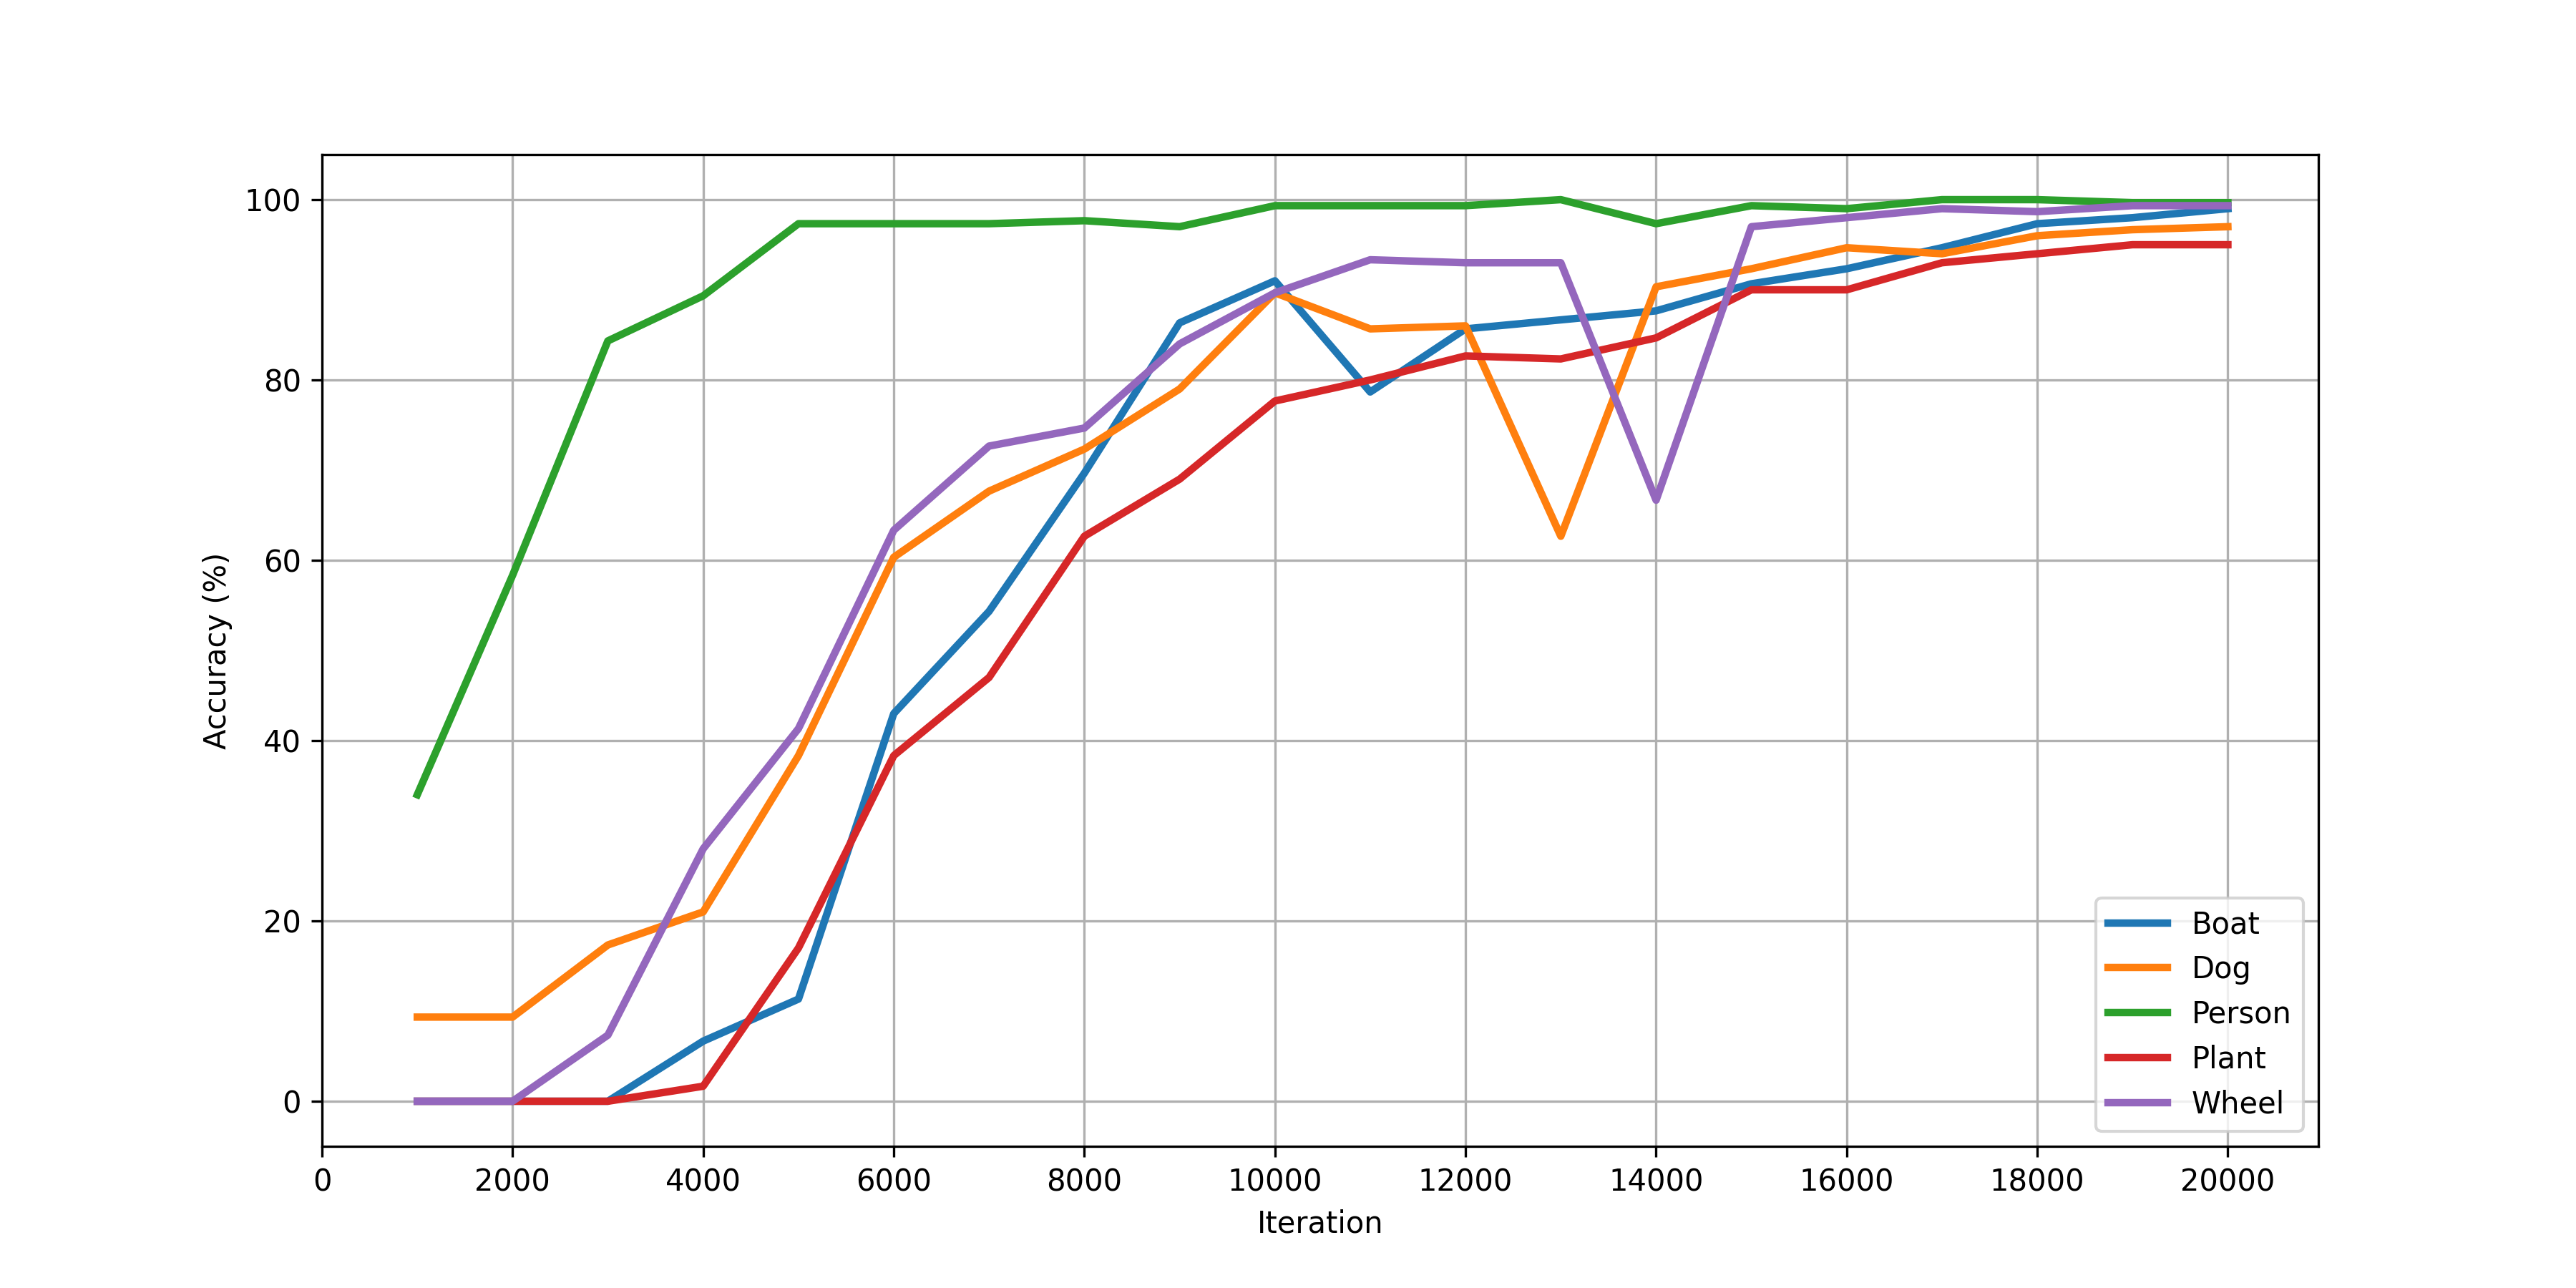
\includegraphics[width=0.9\textwidth]{../Data/accuracy-graph.png}
   \caption{Accuracy per Class over 20,000 Training Iterations}
   \label{fig:accuracy-vs-training-iterations}
\end{figure}


To assess the overall performance of the model, the average accuracy per iteration and its rate of change were calculated.
The "Average Accuracy" in Figure \ref{fig:accuracy-improvement} displays the aggregated information seen in Figure 
\ref{fig:accuracy-vs-training-iterations}. The aggregation of data attenuates the fluctuation seen for the classes "Dog" and "Wheel" 
(See Fig. \ref{fig:accuracy-vs-training-iterations}) and thus making the the upward trend between 10,000 and 20,000 iterations more visible.
\\
The model starts off with a substantial increase in accuracy, which is followed by a dip in the rate of change, as the rise in accuracy 
decelerates. A further steep incline can be detected between 4000 and 6000 iterations, which is followed by a steady increase in accuracy, as
the rate of change falls. A small dip in accuracy can be seen at iteration 11,000, after which a bigger anomaly occurs between 13,000
and 14,000 iterations. Following the dip, the model resumes its positive uptrend trend, reaching an average performance of 98\% after its final
iteration (20,000).
\newpage

\begin{figure}[h]
   \centering
   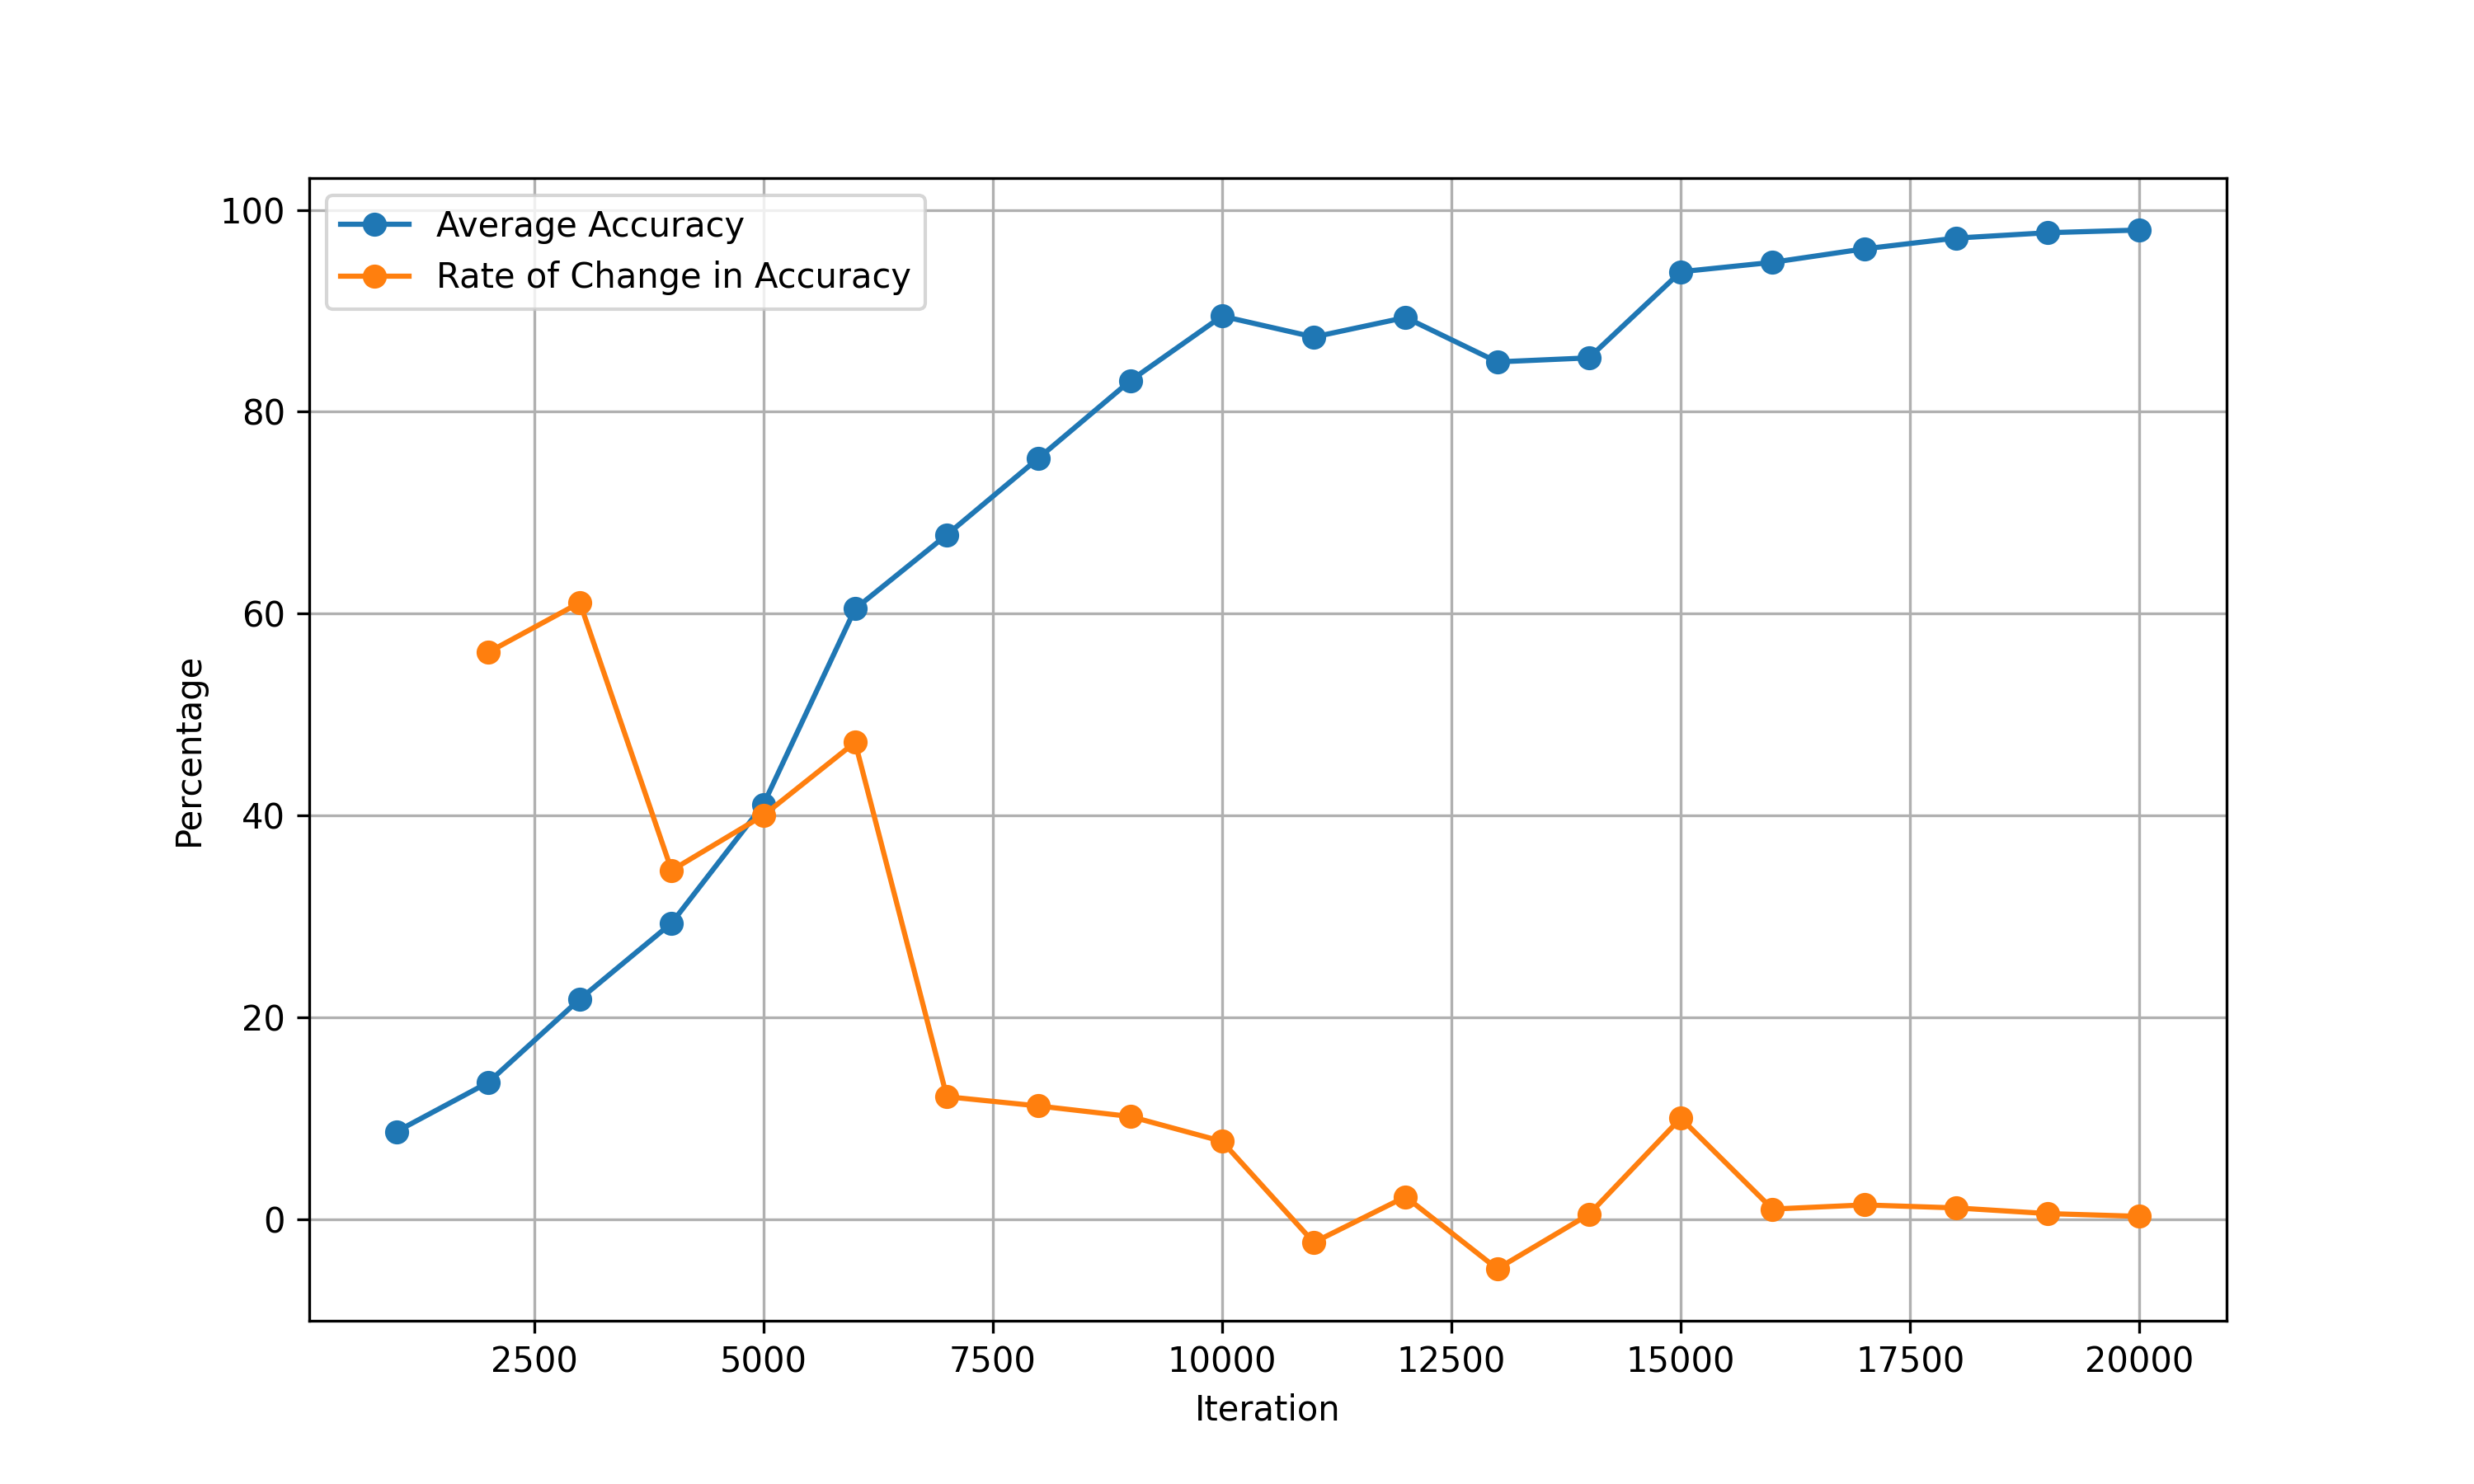
\includegraphics[width=0.9\textwidth]{../Data/accuracy-improvement-graph.png}
   \caption{Average Accuracy and its Rate of Change}
   \label{fig:accuracy-improvement}
\end{figure}

Overall, the chart depicts a generally positive trajectory for the average accuracy, with a few outliers. The "Rate of Change" emphasizes
key points in the model's learning process and makes instances in which the average accuracy experiences notable increases or decreases more
visible. The described fluctuation in accuracy needed to be further investigated, hinting at possible
challenges in the learning process of the object detection model. \\

\subsection{Analysing fluctuation in loss and accuracy}
- address the outliers, 
- refrence the the accuracy for the diffrent iterations 

- two graphs showing the outlieres

\subsection{Distribution of model accuracy across training iterations}
- box plot per iteration 





